
\section{Fundamentals and Related Work}
\subsection{The PageRank Algorithm}
% Describe how PageRank works: power iteration, damping factor, convergence.



PageRank is an algorithm originally introduced to measure a website's relevance on the World Wide Web. A website's rank is higher the more websites link to it. It was created by Larry Page and Sergey Brin, the founders of Google, to optimize the search engine.
The foundation of the algorithm is a graph where every node represents a website in the internet and an edge translates to a hyperlink on a website.
\begin{figure}[ht]
    \centering
    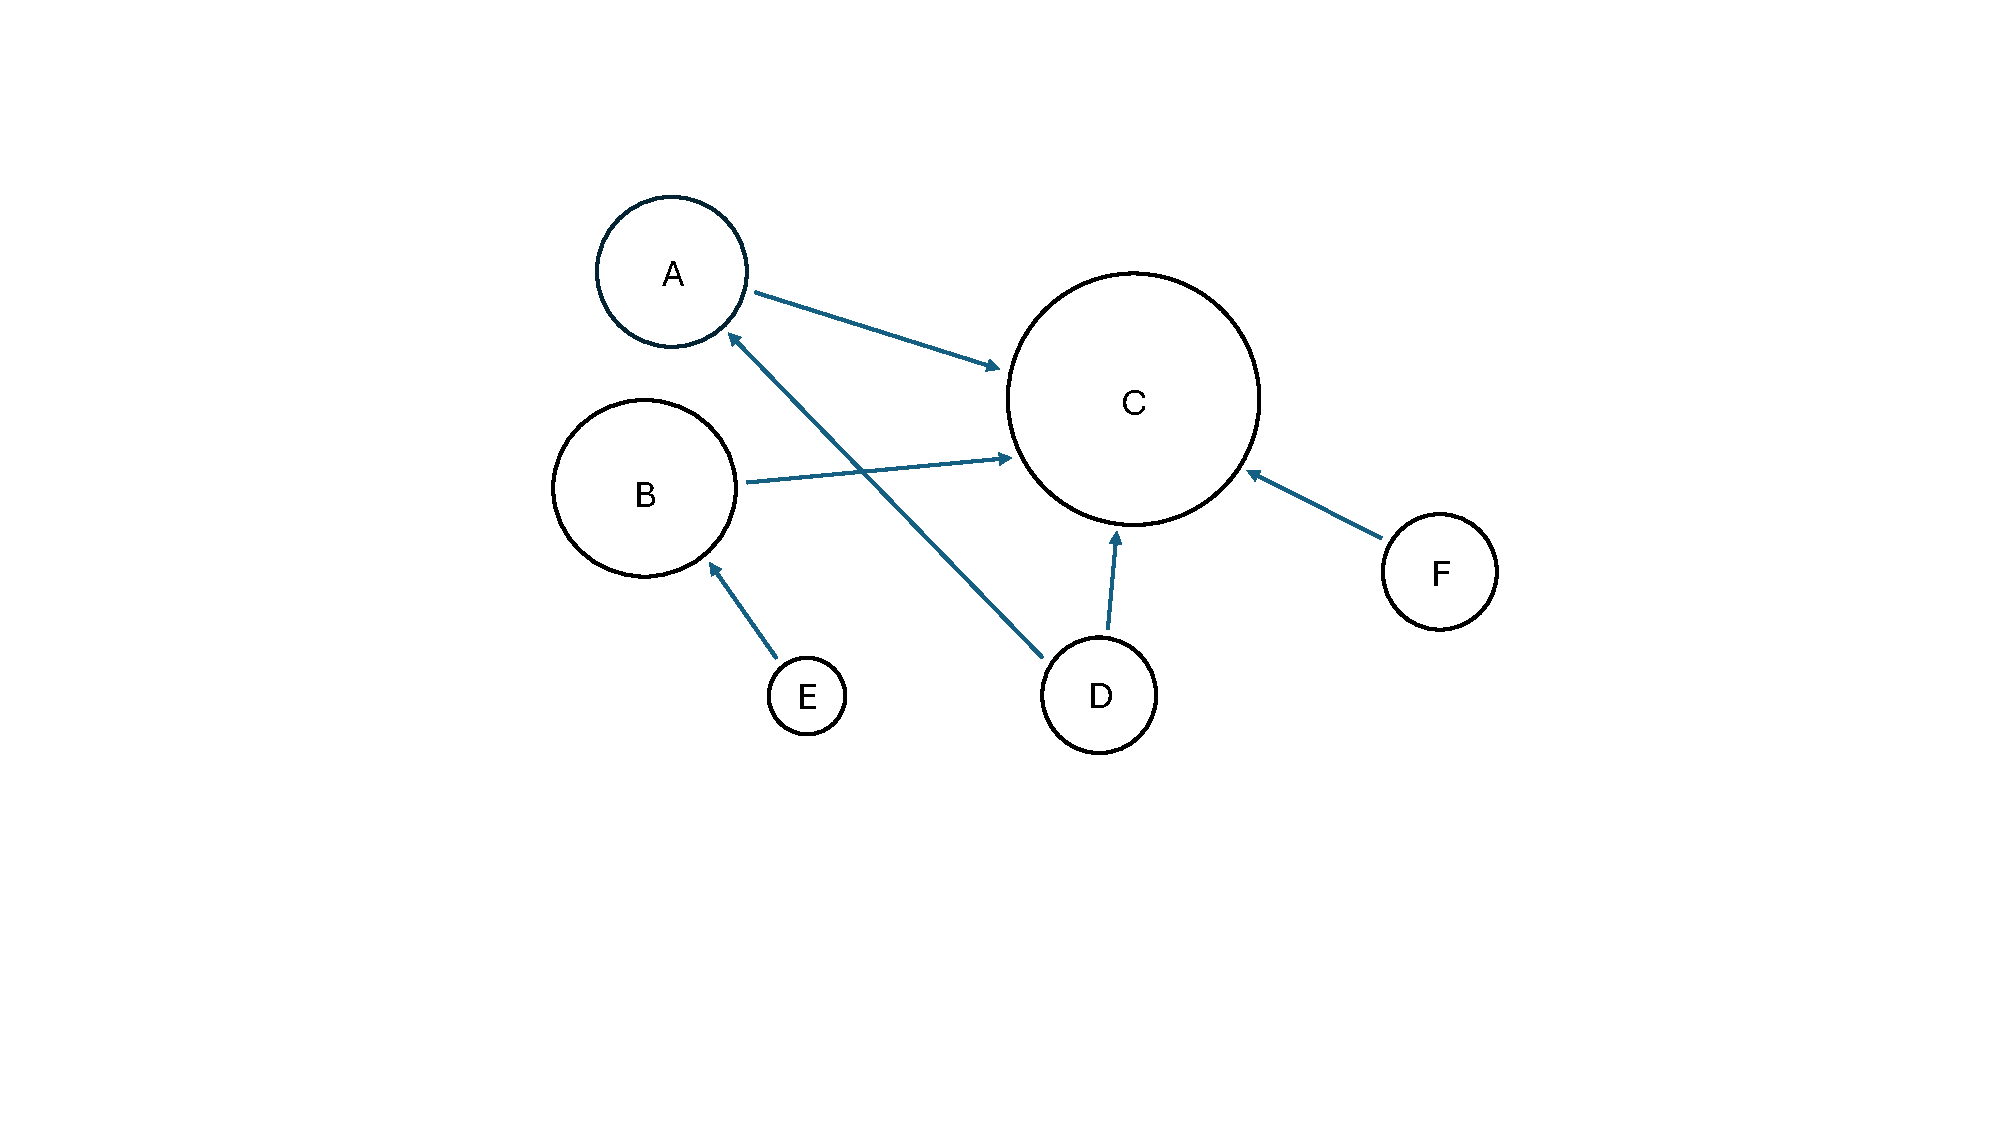
\includegraphics[width=0.7\linewidth]{images/PageRank Graph.pdf}
    \caption{PageRank Graph}
    \label{fig:pagerank-toy}
\end{figure}

To calculate the PageRank values, a transition matrix is constructed, in which each row represents a state, a website, and contains the probabilities of moving from one node to another. In figure 1 D has two outgoing edges, so the probability of moving from D to another node is $0.5$. The transition matrix describes the behavior of a "random surfer". The random surfer model describes the probability of a random user visiting a website. Finding the PageRank values is a Markov chain process, and its stationary distribution is the PageRank vector. Additionally, to model realistic user behavior, a damping factor is introduced, which is commonly set to 0.85. That means with probability $\alpha$ a random surfer clicks on an outgoing hyperlink on the current website and with probability $1-\alpha$ the surfer "teleports" to a random website in the graph. This characteristic is necessary for PageRank because web graphs can have dangling nodes, disconnected parts or cycles. Thus, the damping factor ensures that the Markov chain is irreducible and aperiodic, which guarantees a convergence to a unique stationary distribution. 
The PageRank algorithm is commonly defined as the following:
\begin{equation}
    \pi_v = \frac{1-\alpha}{n}+c\sum_{u\in N^-(v)}\frac{\pi_u}{d^+(u)} \quad\text{\cite{chebolu_pagerank_2008},}
\end{equation} 
where: 
\begin{itemize}
    \item $\pi_v$ is the PageRank of the node $v$
    \item $\alpha$ is the damping factor
    \item $n$ is the total number of nodes in the graph
    \item $N^-(v)$ is the set of ingoing edges of $v$
    \item $d^+(u)$ is the out degree of $u$
\end{itemize} 
% talk about tolerance and convergence
The calculation of PageRank follows the power iteration method, a technique to finding the dominant eigenvalue. The iterative process is defined as follows
\begin{enumerate}
    \item Define the initial vector 
    \begin{equation}
        \pi^{(0)}=\frac{1}{n}e
    \end{equation}
    \item At each iteration apply the update rule, where $S$ is the transition matrix and $e$ is the all-ones vector
    \begin{equation}
        \pi^{(k+1)} = \alpha S^T+ \frac{(1-\alpha)}{n}e
    \end{equation}
    \item Continue until the difference between iterations is less than a tolerance $\epsilon$
    \begin{equation}
        ||\pi^{(k+1)}-\pi^{(k)}||_1<\epsilon \quad \text{\cite{langville_googles_2012}\cite{page_pagerank_1999}}
    \end{equation}
    
\end{enumerate}
Then $\pi$ satisfies 
\begin{equation}
    \pi=G^T\pi, \quad \text{where $G=\alpha S +\frac{1-\alpha}{n}ee^T$}
\end{equation}
and $\pi$ is a stationary probability distribution, the unique PageRank vector.
Each entry in the PageRank vector represents the probability that a random surfer will land on a specific node. The power iteration method has a time complexity of $O(m)$ per iteration, where $m$ is the the number of edges. Thus, the total complexity is $O(m\cdot k)$. The number of iterations $k$ depends on the damping factor ,$\alpha$, and the tolerance ,$\epsilon$. After the original PageRank algorithm has been introduced many more variants have been developed such as personalized PageRank (PPR) \cite{park_survey_2019}.
Here, teleportation is not uniformly distributed across all nodes. Instead, the random surfer only jumps to a specific set of nodes, "restarting nodes". The resulting PageRank vector is a measure of closeness to the restarting nodes in the set \cite{priyanta_social_2019}. 

 
\subsection{Challenges in Large-scale Graph Processing}
% Memory and computational bottlenecks with big graphs
When PageRank was introduced, the number of websites was already estimated to about 150 million. Today even more big graph data is generated by applications such as social networks and communication networks \cite{gebreegziabher_chapter_2023}. Thus analyzing these large-scale graphs has become a significant challenge as memory limitations arise. Since the PageRank algorithm needs to store the whole transition matrix that requires $O(n^2)$ in the worst case, it is not feasible for large graphs with a billion nodes \cite{wu_efficient_2024}. Each iteration requires the whole graph structure in memory and it can take around a hundred iterations to convergence \cite{langville_googles_2012}, with the cost of $O(m)$ per iteration that creates a huge computational overhead. Often a single machine is not enough for large-scale graph analytics tasks due to memory and computing power limitations. On the other hand applying large graphs to distributed systems comes with numerous challenges such as parallelism and load balancing. To address these challenges many distributed graph systems have been proposed to store large graphs in multiple machines and compute algorithms like PageRank  including Pregel \cite{meng_survey_2024}.



\subsection{Apache Spark and GraphX}
% Explain architecture, vertex-centric computation, and limits of GraphX PageRank.


GraphX is a library built on top of Apache Spark that specializes in large graph processing. It provides a powerful Pregel API that can implement the specialized graph parallel system abstraction described in\cite{malewicz_pregel_2010} and a simple representation of data in relational algebra described in \cite{xin_graphx_2014}. Pregel is a specialized graph processing system originally introduced by Google \cite{malewicz_pregel_2010}. It uses a vertex centric technique that follows the philosophy of "think like a vertex", where a graph analytics algorithm iteratively executes a program over vertices \cite{xin_graphx_2014}. 
Specialized systems like Pregel are optimized for graph algorithms, but they are not suitable for practical use since they lack the flexibility to combine graph analysis with broader data processing tasks and the integration of such systems with other data stacks is limited. In contrast, GraphX's integration into Spark's unified analytics platform allows for the seamless combination of graph analytics and other data pipelines. This approach eliminates the need for external ETL integration and data movement, both of which are common with specialized systems. Additionally, GraphX offers optimizations such as vertex-cut partitioning and join elimination, positively impacting communication and runtime \cite{xin_graphx_2014}. Nevertheless, GraphX suffers from the general-purpose nature of the Apache Spark system and may struggle with runtime and very large graphs due to its high memory demand \cite{zhuo_distributed_2021}.  
Finally, GraphX achieves comparable performance to systems like Pregel, while also providing an efficient, end-to-end analytics pipeline. This makes GraphX a more versatile framework for real-world applications \cite{xin_graphx_2014}.

\subsection{Spark's Memory Management}
Apache Spark's memory allocation is crucial for good performance of Spark applications. Spark uses a unified memory, the JVM Heap Space, which is also called as Spark Executor Heap Space. The amount of JVM Heap Memory allocated to each executor is called spark.executor.memory. It is distributed further into three parts: 

\begin{figure}[ht]
    \centering
    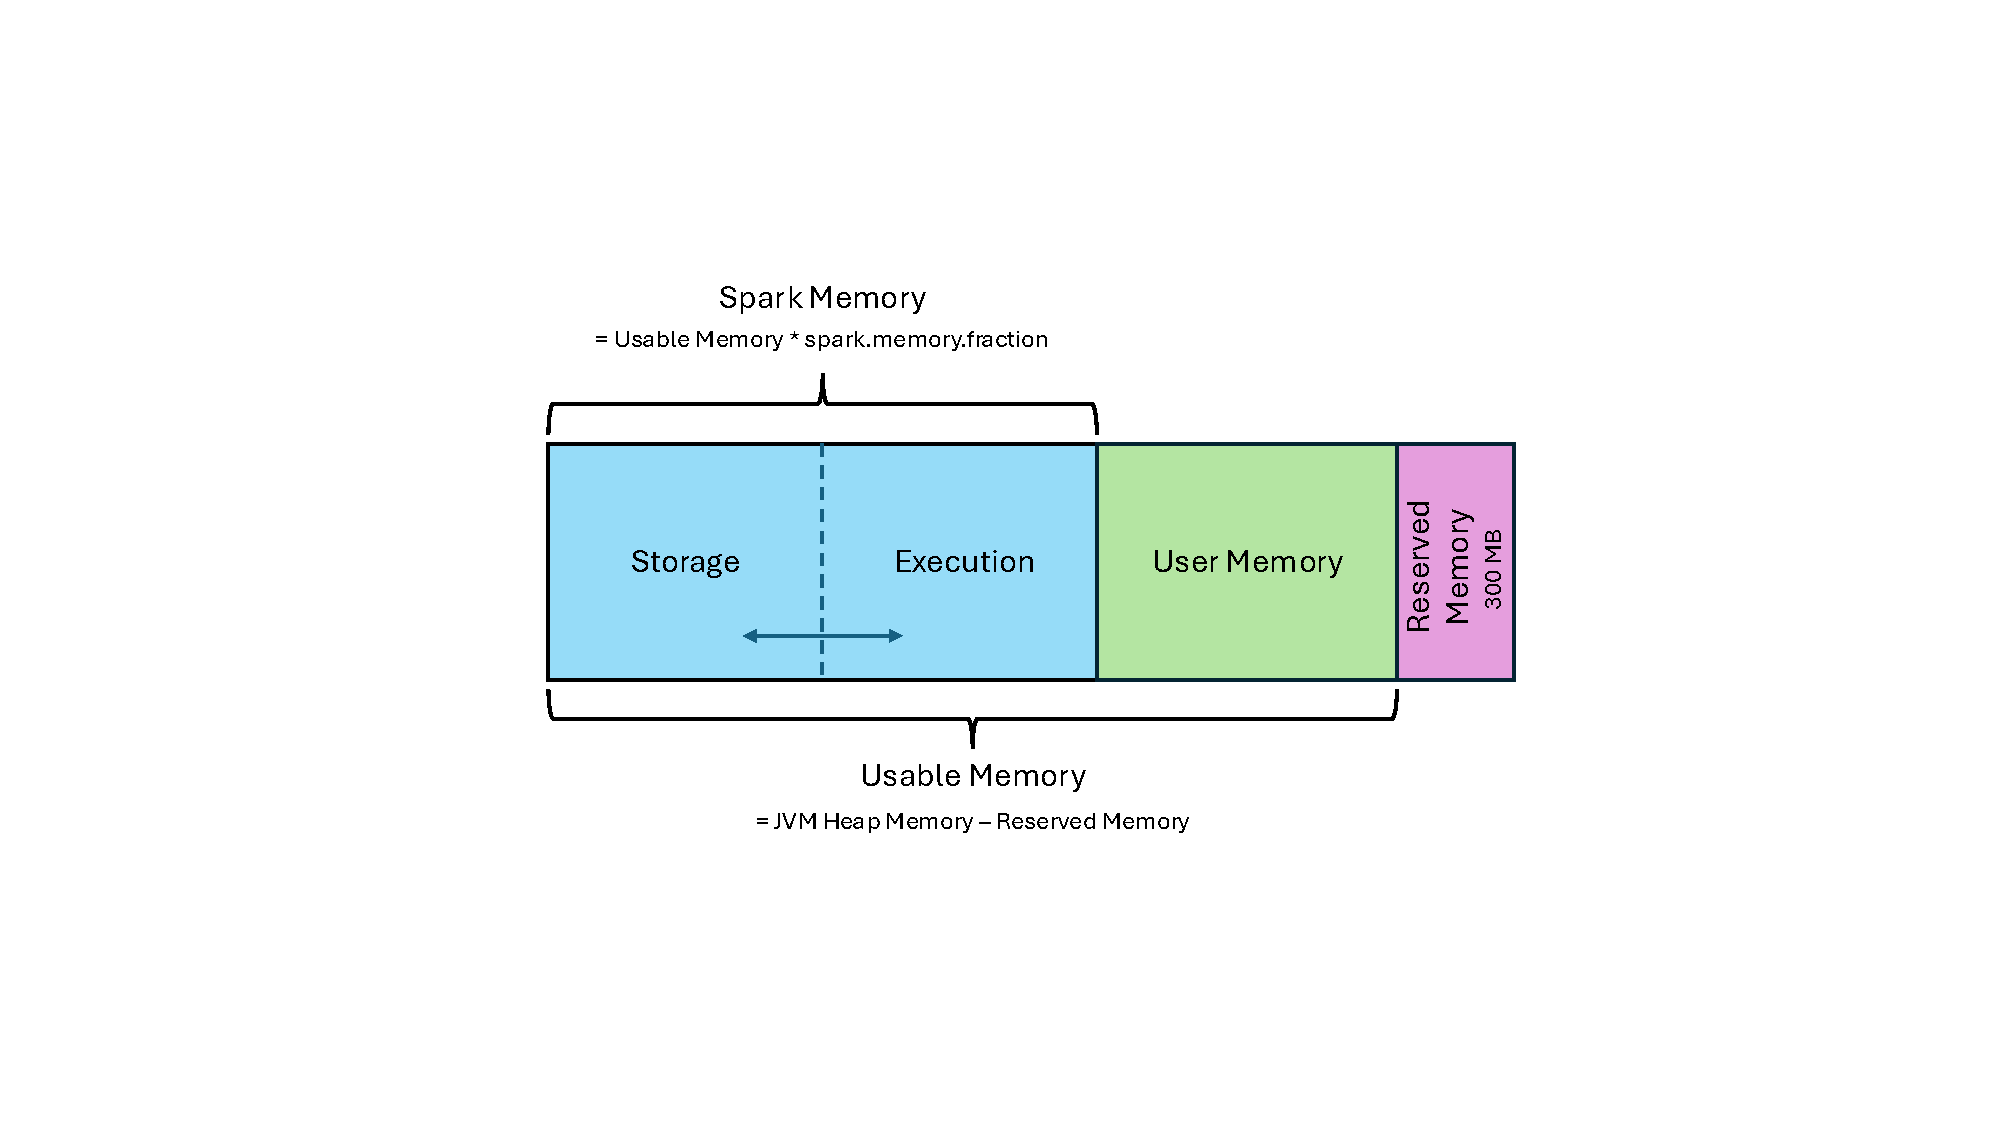
\includegraphics[width=0.7\linewidth]{images/Spark_mem_man.pdf}
    \caption{JVM Heap Memory}
    \label{fig:spark-mem-man}
\end{figure}

\textbf{Reserved Memory.} Out of the total memory allocated to an executor, 300 MB are reserved to store Spark internal objects. It is constant overall executors and guarantees sufficient memory for the system \cite{apache_spark_configuration_2025}.
\textbf{Spark Unified Memory.} This section is the usable memory, divided into two subregions: \textbf{Spark Memory} and \textbf{User Memory}. The memory allocation depends on spark.memory.fraction. Typically, $60\%$ of the memory is allocated to Spark Memory and $40\%$ to User Memory. Forty percent of the user memory is used to store user data and the results of operations. The Spark Memory consists of execution and storage memory. While execution memory is mainly used to store temporary data for all computations such as shuffles, joins and aggregations, storage memory holds cached data, broadcast variables. Furthermore the memory allocation between the two can be configured through spark.memory.storage.Fraction where the default value is $0.5$. A special feature of Spark memory is that it's flexible, Spark allows executor and storage memory to borrow from each other. This is called dynamic occupancy mechanism. But this feature comes with some restraints: While storage memory can borrow as much execution memory when it's not used, execution memory can only borrow memory up to a certain threshold called onHeapStorageSize. This part is only used by storage memory when its not occupied by execution memory. Storage memory can not evict execution memory and has to wait until it's free. On the other side execution memory has priority and is able to evict borrowed memory. In that case cached data will evicted until sufficient memory is released. This is because executing a task is more critical than the cached data. A task can fail if the execution is OOM. Although, most operations are executed in on-heap memory, which is subject to garbage collection (GC), Spark has the possibility to move certain operations to off-heap memory, which reduces GC overhead. Here memory is stored outside the JVM heap, allowing Spark to manage memory more efficiently. It can improve performance for lagrger workloads but it adds a layer of complexity since Spark needs to handle memory allocation and deallocation \cite{chambers_spark_2018}\cite{apache_spark_tuning_2025}. 

\subsection{Resilient Distributed Dataset}
Resilient Distributed Dataset (RDD) is the core abstraction in Spark. An RDD is a partitioned collection of elements that is distributed across the nodes of a cluster and that is processed in parallel \cite{apache_spark_rdd_2025}. RDD's are immutable and resilient to failures due to lineage, which is a feature that records all transformations applied to the data. In case of a node failure the lost data can be recomputed with the help of records. There are two types of operations that RDD's can do: transformations and actions. With each transformation such as map, filter, join, a new RDD is created, while an action like  count triggers execution. RDD's can be cached or persisted in memory to avoid recomputation in each iteration \cite{chambers_spark_2018}. Since RDD's are immutable, every transformation creates a new RDD's, which easily creates high memory usage, especially when computing iterative graph algorithms such as PageRank, where each iteration creates new RDD's for vertex properties. 



\subsection{Approximate PageRank Methods}
% Iteration, sampling, matrix approximation, and Monte Carlo approaches.

The standard PageRank method uses power iteration, which requires storing the entire graph structure in memory and updating the PageRank values with each iteration until convergence. For large graphs, this this process is computationally and memory intensive, making it infeasible in practice. Therefore, approximate PageRank algorithms have been proposed for practical large-scale analysis that trade off accuracy for efficiency \cite{wu_efficient_2024}. The following methods have been introduced:
\textbf{Iteration methods} \cite{xie_parameterized_2023-1}\cite{anikin_efficient_2022} accelerate the standard power iteration but still operate on the whole graph structure \cite{wu_efficient_2024}. 
\textbf{Sampling-based methods} estimate PageRank values by using smaller, sampled subgraphs \cite{bar-yossef_local_2008}\cite{chen_local_2004}. Despite reducing the size of the input data, these methods cannot estimate the PageRank values for the vertices outside the sampled set \cite{wu_efficient_2024}.
\textbf{Matrix approximation methods} use a low-rank approximated transition matrix to estimate PageRank values \cite{liu_fast_2015}\cite{benczur_feasibility_2005}. 
\textbf{Monte Carlo methods} estimate PageRank by simulating random walks on the graph. Instead of iteratively updating a full rank vector, these models simulate many random walks on the graph \cite{avrachenkov_monte_2007}. The value of a node is estimated by the number of walks that end at the vertex. In order to achieve high accuracy, these methods have to go through a large number of iterations \cite{wu_efficient_2024}. However, the memory required during the simulation can be controlled by the number of concurrent random walkers rather than by the total number of vertices \cite{avrachenkov_monte_2007}. Given the potential memory advantages by controlling the random walker count, Monte Carlo methods offer a promising direction for large-scale PageRank approximation.